\chapter{Producto de datos}

\noindent Este capítulo tiene el propósito de describir el producto de datos desarrollado con referencia a la Edición XII (2019-2019) del Estudio Anual de AMAI, para lo cual se ha dividido en tres secciones. La primera de ellas brinda un \emph{overview} de dicho producto de datos, el segundo versa sobre la descripción del \emph{pipeline} que le da sustento y finalmente la tercera sección aborda la descripción técnica del producto de datos.

\section{Overview del producto de datos}

El producto de datos del proyecto consiste en un proceso automatizado para realizar los cálculos que permiten dar respuesta los objetivos de negocio descritos en las secciones \ref{obj:bussiness} y \ref{obj:datascience}, a partir de la bases de datos históricas que reúnen las respuestas de las empresas al Estudio Anual de AMAI, plasmando sus resultados en reportes documentos dirigidos al público y a los participantes del estudio,los cuales son relevantes para analizar la situación que prevalece en el mercado mexicano de investigación e inteligencia aplicada a mercados, medios y opinión pública.

En concreto, con referencia a la Edición XXII del Estudio Anual de la Industria de Investigación de Mercados y Opinión Pública en México, dicho proceso se ha usado para consolidar dos documentos, a manera de reportes ejecutivos, que permiten exponer al público en general y, de manera confidencial, a los participantes del estudio los principales hallazgos facilitando   su   entendimiento   y   ayudando   a   encontrar elementos de valor para la industria.

A continuación se ofrece una descripción detalla del proceso que se ha diseñado para tal efecto.

\section{Descripción del pipeline}\label{dataproduct:process}

Como se ha mencionado, el Centro de Ciencia de Datos ITAM recibió la información histórica de los estudios realizados previamente, incluyendo las respuestas de las empresas informantes, así como los  correspondientes reportes anuales en formato de hojas de cálculo en MS Excel, cuyo contenido principalmente es relativo a respuestas en valores numéricos, porcentajes y texto libre. Bajo la consideración de que tal información se ha reunido hasta la fecha más reciente el pipeline de este proyecto se puede describir como sigue: 

\begin{itemize}
     \item \textit{Raw Schema:} Carga de información contenida en las hojas de cálculo se cargó hacia esquemas crudo de PostgreSQL, sin realizar modificaciones de ningún tipo.
    
    \item \textit{Clean Schema:} corresponde a una serie de acciones de limpieza de las fuentes de datos, entre las que destacaron 1) cambiar el texto a minúsculas, 2) eliminar acentos, guiones, espacios,  y 3) corregir lectura de caracteres raros debidos a codificaciones no identificadas. A su vez, cabe destacar que, ante la ausencia de llaves, en este punto se procede a identificar al nombre de las empresas como columna común a las bases de datos de las diferentes ediciones del Estudio Anual de AMAI para poder cruzar información de diferentes periodos\footnote{Dicho punto fue especialmente problemático dado que ante la ausencia de mecanismos de control el llenado de información de los participantes, una misma empresa podía presentase con nombres ligeramente distintos en periodos diferentes lo que complica su identificación desde el texto (por ejemplo, con abreviaciones, denominaciones comerciales o legales), para lo cual se procedió a homologan los nombres correspondientes.}.
    
    \item \textit{Bussiness Calculations:} Corresponde a la ejecución de cálculos o procesamientos de las fuentes de datos limpias para dar respuestas a los objetivos descritos en las secciones \ref{obj:bussiness} y \ref{obj:datascience}, a través de scripts del lenguaje SQL, los cuales son importados hacia R para alimentar los correspondientes reportes ejecutivos hacia AMAI (es decir, la versión dirigida al público y la versión confidencial para a participantes de la Edición XXII del Estudio Anual de AMAI)\footnote{Cabe destacar que en el caso de conteos o cálculo de distribuciones porcentuales con respecto a alguna variable, a menos que se indique lo contrario, se contabilizan únicamente respuestas explícitas, es decir, no se llevaron a cabo imputaciones de datos ante la ausencia de respuesta de un participante.}. 
\end{itemize}

Para facilitar el entendimiento del proceso recién descrito, este se ha representado a través del siguiente diagrama:

\begin{figure}[H]
\begin{center}
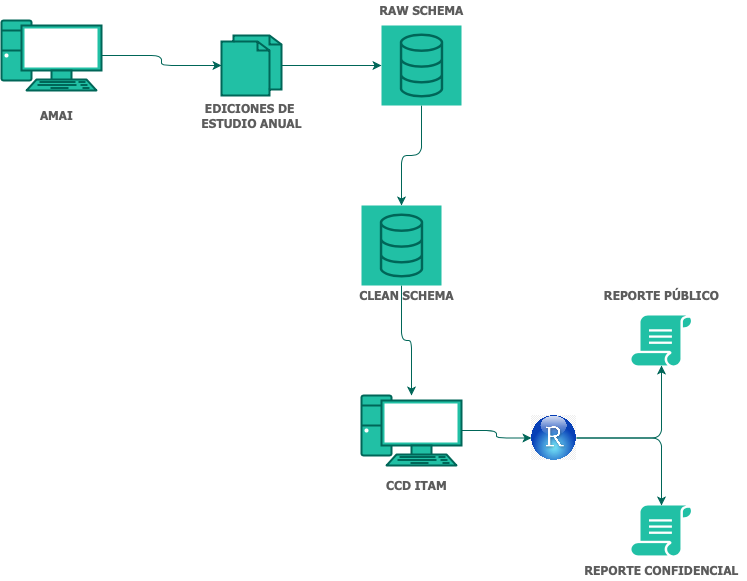
\includegraphics[scale=0.4]{Imagenes/pipeline.png}
\end{center}
\caption{Pipeline del producto de datos materia del proyecto con motivo de la Edición XXII del Estudio de AMAI}
\end{figure}
\

\section{Consideraciones éticas del producto de datos}

Teniendo presente la importancia para la industria de la información recabada en el marco de la Edición XXII (2019-2019) del Estudio Anual de la Industria de Investigación de Mercados y Opinión Pública en México y la sensibilidad de la misma, se realizó el procesamiento y análisis de la información recibida preservando el carácter confidencial de la misma. Para ello, de manera específica se destaca que:

\begin{itemize}
 \item Los datos fueron procesados sin revelar a ninguno de los participantes terceros el contenido de las respuestas del estudio, de manera directa o indirecta.
 \item  La información reunida se empleó para estimaciones o conteos de forma agregada, sin exponer los datos reportados individualmente por las empresas ni sus correspondientes identidades.
 \end{itemize}

\section{Descripción técnica de producto de datos}

La presente sección brinda la descripción a nivel técnico del producto de datos considera el procesamiento de la información, las consideraciones metodológicas y la solución tecnológica establecida para su desarrollo.

\subsection{Consideraciones metodológicas}

A continuación se exponen las consideraciones metodológicas tomadas en cuenta para consolidar los objetivos de negocios descritos en las secciones \ref{obj:bussiness} y \ref{obj:datascience}. Cabe destacar que estos fueron recogidos a su vez y publicados por AMAI en el documento \emph{Estudio AMAI Edicion XXII (2019-2020). Nota Metodológica.}\footnote{Véase \url{http://amai.org/descargas/reporteMetodologicoCliente270520.pdf}}

\subsubsection{Generalidades}

Tal como se ha expresado en la sección \ref{dataproduct:process}, 
por lo que hace a la identificación de los participantes en el Estudio Anual de AMAI a lo largo del tiempo, ésta se realizó con base en una versión homologada del nombre de las empresas. 

\subsubsection{Tamaño del mercado}

En línea con la metodología por AMAI en estudios previos, el dimensionamiento del tamaño del mercado se realizó con base en la facturación (en pesos  mexicanos) de las empresas que conforman el sector de inteligencia de mercado y  opinión para el periodo del estudio. Sobre este punto, la estimación consideró la suma de tres diferentes componentes relativos al tamaño de mercado \emph{calculado}, \emph{estimado} y \emph{supuesto}:

\begin{itemize}
    \item \emph{Calculado:} se refiere a los datos de facturación que fueron proporcionados explícitamente por los informantes en el contexto del estudio,
    \item \emph{Estimado:} relativo a la información de facturación que aunque no fue proporcionada de forma explícita, se tienen datos históricos u otras fuentes que permiten estimarlos en el periodo relevante.
    \item \emph{Supuesto}: corresponde al resto de la industria sobre lo cual se desconocen los datos de facturación.
\end{itemize}

A continuación se describe la metodología adoptada en cada uno de tales
conceptos:\vspace{0.5cm}

\noindent \emph{Metodología para el valor de mercado calculado}

\noindent Se estima como la suma del nivel de facturación reportado por los participantes.\\

\noindent \emph{Metodología para el valor de mercado estimado}

\noindent En primera, se identificaron empresas que 1) contestaron el estudio sin proporcionar datos de facturación, o bien 2) dejaron de participar en dicho  estudio debido a algún motivo y que, por ende, se dejó de tener datos de su facturación en ésta edición.

Posteriormente, se hizo una análisis de la información histórica reunida por AMAI de tales empresas, para identificar los valores de facturación más recientes de los que tuviera noticia para tales empresas, encontrándose que para la mayoría de empresas bajo los supuestos 1) y 2), existen registros de su nivel de facturación en la edición 2018. Sin embargo, para dos empresas los datos encontrados se ubican en periodos más lejanos.

En consideración de ello, para el caso de las empresas donde existe información de su facturación en 2018, el nivel correspondiente al 2019 se estimó aplicando al valor 2018 una tasa ponderada de cambio en el nivel de facturación de ambos periodos, cuyo cálculo se realizó con base en la mediana, en términos porcentuales, de la variación observada sobre la facturación de las empresas para los que si se encontraron datos en 2018 y 2019 (es decir, empresas coincidentes 2018-2019). Esta tasa fue cuantificada en $-3.6\%$.

Se consideró pertinente emplear dicha tasa dada la dinámica observada en el nivel facturación de las empresas coincidentes de 2018 y 2019, la cual se ejemplifica en la figura 3.1, donde se han modificado los nombres de las empresas para respetar los acuerdos de confidencialidad existentes entre AMAI y el CCD del ITAM.

\begin{figure}[h]
\begin{center}
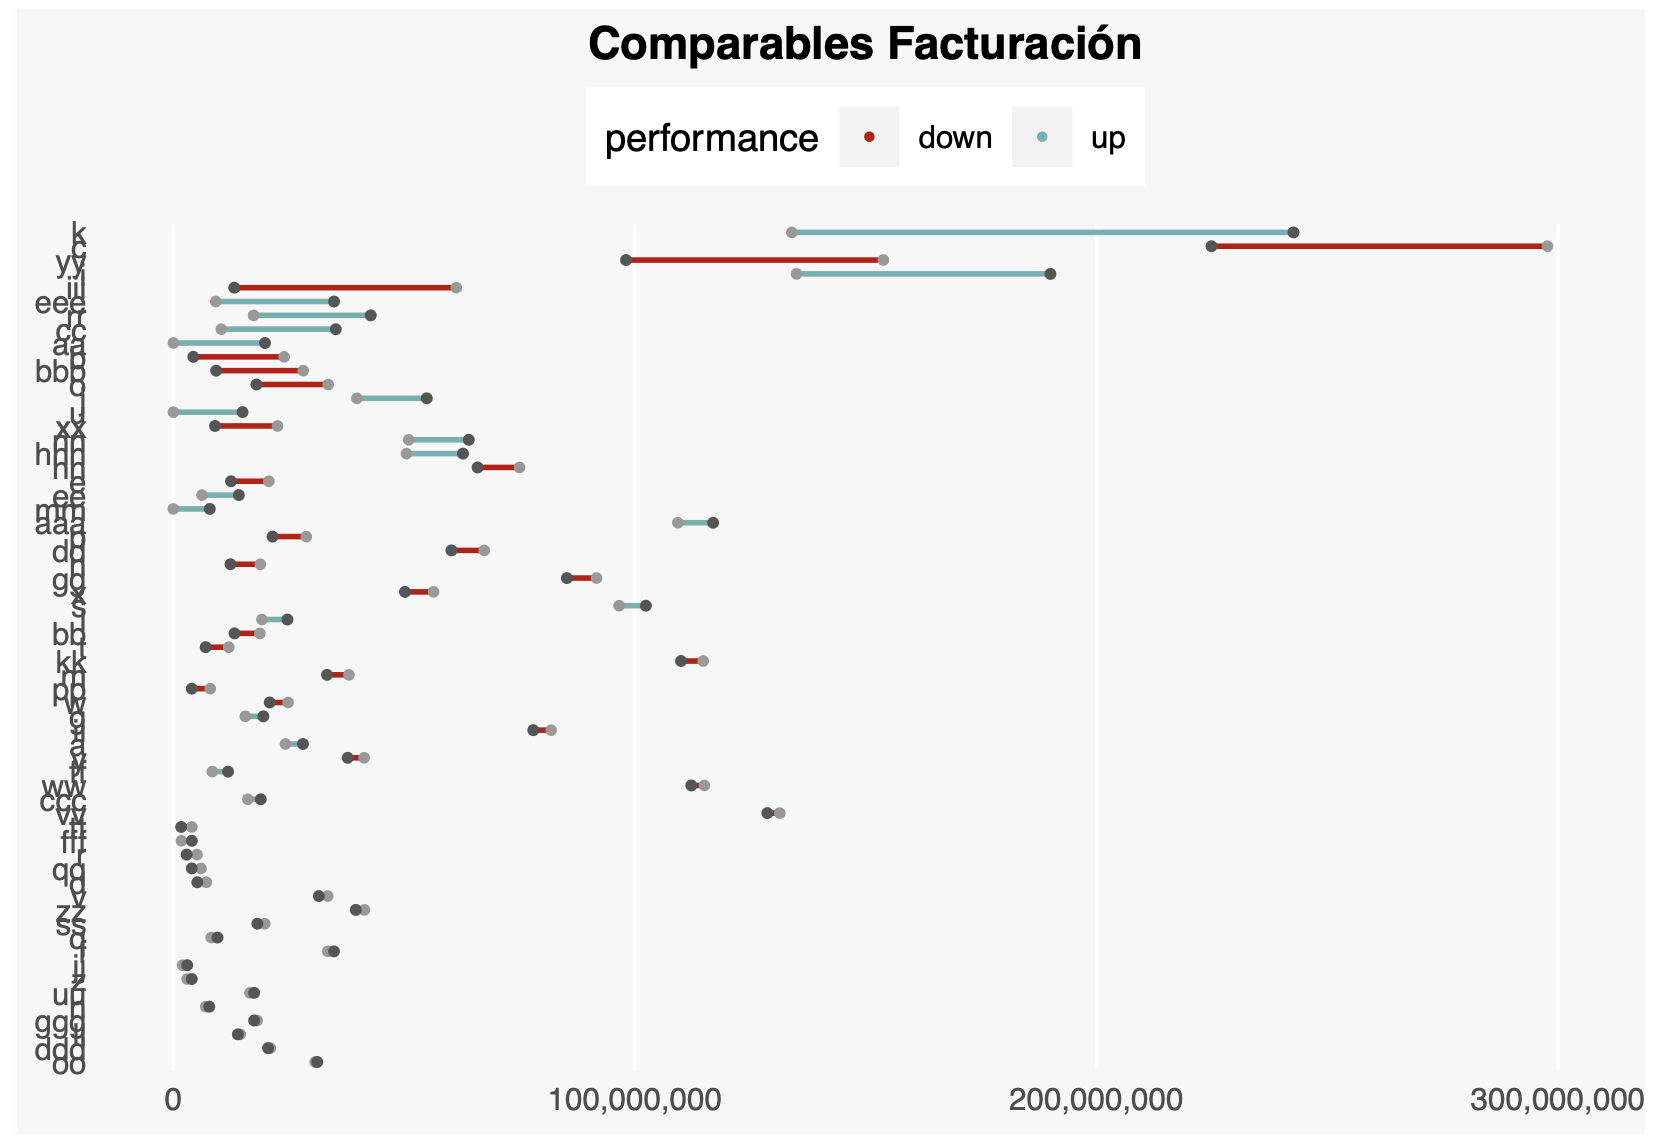
\includegraphics[scale=0.4]{Imagenes/empresas_coincidentes.png}
\end{center}
\caption{Comparación de niveles de facturación de empresas coincidentes 2018-2019 en ambos periodos}
\end{figure}

\newpage

Por otra parte, se hicieron consideraciones particulares sobre dos empresas:

\begin{itemize}
\item En el primer caso se identificó que el último dato de facturación existente se remonta a 2015. Sin embargo, éste valor es menor, en tres órdenes de magnitud, al resto de información histórica de dicha empresa. Ante la evidencia, se consideró que probablemente fue un error de llenado en los datos de facturación para esta empresa, por lo que para 2015 dicho valor se  ajustó multiplicándolo con un factor de 1,000. Adicionalmente, para poder estimar su facturación correspondiente a 2019, sobre el dato de 2015 se aplicaron, de manera consistente con la metodología de AMAI en el estudio 2018, una serie de tasas de crecimiento anual de dicha empresa que fueron reportadas verbalmente a AMAI (9\% a 2016, 8\% a 2017 y 6\% a 2019), así como el valor estimado de crecimiento de facturación de las empresas en el estudio previo (4.7\% a 2018).
\item Para el segundo caso, se identificó que el último valor de facturación reportado corresponde a 2017. En este caso, el valor correspondiente a 2019 se estimó aplicando una tasa ponderada de cambio en el nivel de facturación, empleando la mediana de la variación observada sobre la facturación de las empresas para los que si se encontraron datos en dichos periodos de a) 2017 a 2018 (2\%), y b) 2018 a 2019 (-3.6\%).
\end{itemize}

\noindent \emph{Metodología para el valor de mercado supuesto}

\noindent Se empleó el mismo procedimiento seguido por AMAI en la edición previa del estudio, relativa considerar que la suma  del valor \emph{calculado} y \emph{estimado} equivale al 80\% del mercado total y que, por ende, el mercado \emph{supuesto} se puede obtener como el complemento, es decir, corresponde a 20\% de la facturación de mercado total.

\subsubsection{Mismas empresas reportando}

Dado que sobre este punto, el interés es comparar los cambios en los niveles de facturación para 2018 y 2018, aquí se tomó como referencia a las empresas que reportaron información de facturación en el periodo 2019 del estudio y en el previo.

A continuación se describe la metodología seguida para realizar comparativos de interés al respecto.\\

\noindent \emph{Diferencias vs año anterior}

Estimado como la diferencia numérica en los datos de facturación de 2018 y 2019, para las empresas coincidentes en ambos periodos.\\

\noindent \emph{Desempeño vs año anterior}

Calculado como la diferencia porcentual entre los datos de facturación de 2018 y 2019, para las empresas coincidentes en ambos periodos.

\subsubsection{Valor de tamaño de mercado}

\begin{itemize}
\item Para los datos de periodos hasta 2018, se empleó la información histórica generada por AMAI en las ediciones pasadas del estudio.

\item Para 2019, se tomó como referencia al proceso descrito en el apartado \textbf{Tamaño del mercado} de la presente sección para el dimensionamiento del tamaño del mercado.
\end{itemize}

\noindent \emph{Tendencia de valor nominal y real de la industria}

En línea con la metodología desarrollada en la edición pasada del estudio, para estimar el valor del tamaño del mercado en términos reales, se realizaron los siguientes pasos:

\begin{itemize}
    \item El valor nominal se consideró de acuerdo al valor estimado de dicha cantidad para 2019, conforme a la exposición realizada en el apartado \textbf{Tamaño del mercado} de la presente sección,
    \item El índice nacional de precios al consumidor publicado por el Instituto Nacional de Estadística y Geografía (INEGI), con base en la segunda quincena de julio de 2018\footnote{Disponible a través de la dirección electrónica \url{https://www.inegi.org.mx/sistemas/bie/}, mediante
la ruta \textit{Indicadores económicos de coyuntura, Índices de precios , Índice nacional de precios al consumidor. Base segunda quincena de julio de 2018=100, Mensual, Índice, Índice general}}.
\end{itemize}

\noindent \emph{Variaciones porcentuales anuales en el valor de la industria}

El cálculo de este punto se estimó como la diferencia porcentual entre los datos de valor de mercado, en términos nominales, de 2013 a 2019, con diferencia de un año. En tal sentido, para el valor nominal del mercado se consideró lo siguiente:

\begin{itemize}
\item  Hasta 2018, se emplearon los datos del valor del mercado estimado en los estudios de AMAI, 
\item  Para 2019, se usó la estimación del CCD del ITAM, conforme al proceso descrito en el apartado \textbf{Tamaño del mercado} de la presente sección.
\end{itemize}

\noindent \emph{Variaciones porcentuales anuales (mismas empresas reportando)}

Análogamente, este punto fue estimado como la diferencia porcentual entre los datos de facturación agregada las empresas coincidentes periodos con diferencia de un año, considerando datos que abarcan de 2013 a 2019. Por lo que hace a los datos del valor nominal del mercado se consideró lo siguiente:

\begin{itemize}
\item Para valores el valor nominal hasta 2018, se emplearon los datos del valor del mercado estimado en los estudios de AMAI, 
\item Para 2019, se usó la estimación del CCD del ITAM, conforme al proceso descrito en el apartado \textbf{Tamaño del mercado} de la presente sección.
\end{itemize}

\noindent \emph{Tendencia de valor nominal de la industria (en dólares americanos)}
Valor nominal del mercado:
\begin{itemize}
\item Para valores hasta 2018, se emplearon los datos del valor del mercado estimado en los estudios de AMAI, 
\item Para 2019, se usó la estimación del valor del mercado total, calculada por el CCD del ITAM para 2019 con la metodología descrita en el apartado \textbf{Tamaño del mercado} de la presente sección.
\end{itemize}

\noindent Tipo de cambio dolar americano a pesos mexicanos:

\begin{itemize}
\item Hasta el año 2018, se emplearon datos reportados de tipo de cambio reportados por el Banco Mundial\footnote{Véase \url{https://datos.bancomundial.org/indicador/PA.NUS.FCRF?locations=MX}}

\item En complemento, para la estimación del 2019, se usó como base al \emph{Tipo de cambio (Fix) para solventar obligaciones denominadas en dólares de los EE.UU.A., pagaderas en la República Mexicana} publicado por el Banco de México\footnote{Véase \url{https://www.banxico.org.mx/tipcamb/main.do?page=tip&idioma=sp} }, calculado considerando promedio de los valores promedio reportados en los días de cada mes, al 24/04/2020.

\end{itemize}

\subsubsection{Volumen de mercado}

\noindent \emph{Volumen de producción}

Para este punto, se contabilizó el total cantidad de unidades reportadas por los participantes del estudio, considerando el total del proyectos realizados en la industria, así como el número de 1) sesiones de grupo presenciales o remotas, 2) entrevistas a profundidad y 3) etnografías o aplicaciones de antropología.

En torno a las sesiones de grupo presenciales o remotas, de la revisión a las respuestas se identificó que un participante reportó haber llevado a cabo cerca de 479,000 sesiones. Al contrastarlo, se encontró que i) considerando las sesiones de grupo reportadas por las empresas en su conjunto, dicha cantidad equivaldría al 98\% de las mismas, mientras que ii) 75\% de las empresas en el estudio tiene a lo más 200 sesiones de grupo.

Es así que ante la posibilidad de que el valor aludido fuera un error de captura se excluyó la respuesta del participante en comento para consolidar el conteo de sesiones de grupo presenciales o remotas.\\

\noindent \emph{Tipo de entrevistas}

Con referencia a este rubro, se contabilizaron los diferentes tipo de entrevistas realizadas (a saber, por Internet, cara a cara en domicilios, vía pública, telefónico y salida de casilla), para posteriormente estimar la correspondiente distribución porcentual de los mismos. 

\subsubsection{Capital humano}

Para la estimación de este concepto, se contabilizó la cantidad de recursos humanos reportados por los participantes del estudio en los diversos segmentos que integran una empresa, esto es, socios y altos ejecutivos, personal técnico y de atención a clientes, de apoyo administrativo y equipo de producción, considerando el desglose por género dentro de cada uno de tales segmentos.\\

\noindent \emph{Distribución de capital humano}

A partir de dicha información, se calcula el número total de recursos humanos en la industria junto con su distribución por segmento.

\subsubsection{Ranking de empresas}

Estimado considerando a las empresas que reportaron explícitamente su nivel de facturación en 2019 y que además otorgaron su consentimiento expreso para formar parte del ranking. 

En este sentido, el ranking se formó considerando las posiciones de las empresas ordenadas de mayor a menor según el nivel de facturación reportado para el periodo del estudio, pero sin revelar el dato concreto de facturación de cada empresa para preservar la confidencialidad de dicha información.

\subsubsection{Ante la incertidumbre futura}

\begin{itemize}
\item Con respecto a este punto, se realizó un análisis de texto que permitió identificar los temas que fueron mayormente abordados en las respuestas de los participantes del estudio 2019, como retos, cambios y temas de innovación para la industria.
\item Como resultado, se reportaron 1) los 10 términos más frecuentes, 2) un resumen ejecutivo de los comentarios vertidos por los participantes en torno a los términos más frecuentes, y 3) una nube de palabras para facilitar la exposición del vocabulario empleado por los mismos, donde el tamaño y color de los términos fue proporcional a su frecuencia\footnote{Para este punto, se eliminaron \emph{stopwords} y caracteres de puntuación, considerándose en el ejercicio unigramas y bigramas, empleando las librerias SnowballC, Wordcloud y RColorBrewer de R}.
\end{itemize}

\subsubsection{Perspectivas 2020}

\begin{itemize}
\item Sobre este tema, el estudio 2019 reúne las perspectivas de los informantes a través de diferentes temas: I) Mi empresa, II) México en general, III) Industria en el mundo, IV) Industria en México y  V) Economía personal,
\item Tales perspectivas son consideradas a través de las etiquetas \emph{igual}, \emph{mejor} y \emph{peor} que limitan las respuestas de las empresas,
\item Considerando tales puntos, se realizaron conteos de las mismas para establecer cantidades totales y proporciones de las perspectivas de dichos temas a través del conteo de las respuestas empleando tales etiquetas.
\end{itemize}

\subsection{Consideraciones tecnológicas}

Para el desarrolló de este proyecto hizo uso de infraestructura de servicios de computación en la nube a través del proveedor Amazon Web Services (AWS), contratados por el CCD del ITAM. En concreto se echaron mano de los siguientes:

\begin{enumerate}
    \item \emph{Amazon S3, Amazon Simple Storage Service o Bucket} es un servicio que proporciona una interfaz de almacenamiento de archivos, en donde se depositaron los datos correspondientes a las diferentes ediciones del Estudio Anual de AMAI. 
    \item \emph{Amazon Elastic Compute Cloud  o EC2} el cual consiste en poner a disposición de los usuarios una máquina virtual con diferentes configuraciones de hardware, espacio y sistema operativo. En este caso se empleó una instancia de uso general, con 8 GB de ram, 4 cores y Ubuntu 18.04.4 LTS.
    \item \emph{Amazon Relational Database Service} se trata de un servicio de base de datos relacional; particularmente se empleó un servicio con una base PostgreSQL, a través del cliente \emph{psql} desde conexión SSH hacia la instancia EC2. 
    \item Todos estos servicios se encontraron inmersos dentro de una \emph{Amazon Virtual Private Cloud (VPC)} que proporciona un entorno restringido de trabajo, para garantizar la seguridad de la información y desarrollos realizados.
\end{enumerate}

Para facilitar el entendimiento a continuación se presenta un diagrama\footnote{Elaborado a través de Arcentry, \url{https://arcentry.com/?src=aws}} de los servicios empleados y de su interrelación:

\begin{figure}[h]
\begin{center}
\includegraphics[scale=0.4]{diagrama_aws.png}
\end{center}
\caption{Diagrama de servicios de AWS utilizados por el CCD del ITAM para el proyecto}
\end{figure}